\documentclass[12pt,a4paper]{article}

\usepackage[ngerman]{babel}
\usepackage{fontspec}
\usepackage{tabularx}
\usepackage{graphicx}
\usepackage{geometry}

\usepackage{xcolor}
\usepackage{listings}

\definecolor{commentGreen}{rgb}{0,0.6,0}
\definecolor{mygray}{rgb}{0.5,0.5,0.5}
\definecolor{mymauve}{rgb}{0.58,0,0.82}

\lstset{language=C++,
    basicstyle=\ttfamily,
    keywordstyle=\color{blue}\ttfamily,
    stringstyle=\color{red}\ttfamily,
    commentstyle=\color{commentGreen}\ttfamily,
    morecomment=[l][\color{mygray}]{\#}
}



\geometry{
    left=2cm,
    right=2cm}
\setlength{\parindent}{0pt}

\newcolumntype{L}{>{\raggedright\arraybackslash}X}
\begin{document}

\section{WLib-SPI-Abstraction}

\subsection{Motivation}
    Angenommen man bekommt die Aufgabe einen Treiber für den über SPI angebundenen Chip-XY zu schreiben.
    Damit die Wiederverwendbarkeit des Treibers sichergestellt werden kann sollte er möglichst plattformunabhängig sein.
    Jedoch ist der Featureset und die Bedienung der SPI-Hardware eine stark plattformabhängige Angelegenheit.
    Es empfiehlt sich deshalb die SPI-Kommunikation als ganzes zu Abstrahieren.
    Die Bedienung der SPI-Hardware wird an einen spezialisierten SPI-Hardware-Treiber delegiert.

    WLib-SPI-Abstraction stellt ein solches Interface zur Verfügung.
    Der Treiber für den Chip-XY benutzt es.
    Die spezialisierten SPI-HW-Treiber der unterschiedlichen Plattformen stellen es zur Verfügung.
            
    \begin{figure}[h]
        \centering
        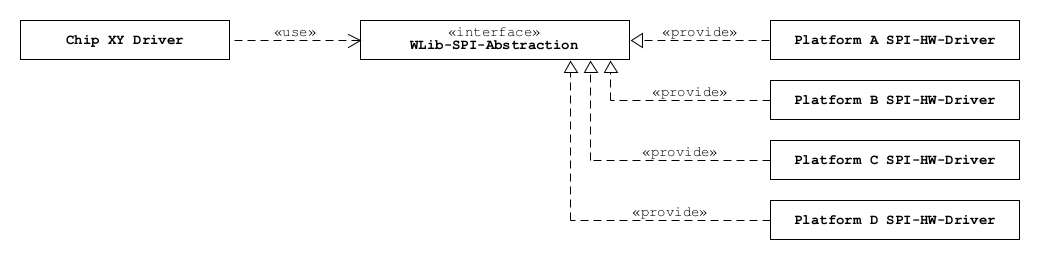
\includegraphics[width=0.7\linewidth]{fig/dependency}
        \caption{Dependency graph}
        \label{fig:dependency}
    \end{figure}
        
        
\subsection{Abstraktes Kommunikationsmodell}

Zuerst wird ein Kommunikationskanal erstellt. Bei der Erstellung des Kanals wird die Hardware konfiguriert.
Der Kanal bietet nun die Möglichkeit durch select_chip das target anzuwählen.
 





\end{document}